\documentclass{article}

\usepackage{booktabs}
\usepackage{tabularx}
\usepackage{hyperref}
\usepackage{listings}
\usepackage{fancyvrb}
\usepackage{geometry}
\usepackage{graphicx}
\usepackage{float}
\geometry{margin=1in}
\graphicspath{ {./images/}}

%% Comments

\usepackage{color}

\newif\ifcomments\commentstrue %displays comments
%\newif\ifcomments\commentsfalse %so that comments do not display

\ifcomments
\newcommand{\authornote}[3]{\textcolor{#1}{[#3 ---#2]}}
\newcommand{\todo}[1]{\textcolor{red}{[TODO: #1]}}
\else
\newcommand{\authornote}[3]{}
\newcommand{\todo}[1]{}
\fi

\newcommand{\wss}[1]{\authornote{blue}{SS}{#1}} 
\newcommand{\plt}[1]{\authornote{magenta}{TPLT}{#1}} %For explanation of the template
\newcommand{\an}[1]{\authornote{cyan}{Author}{#1}}

%% Common Parts

\newcommand{\progname}{Software Engineering} % PUT YOUR PROGRAM NAME HERE
\newcommand{\authname}{Team 2, SyntaxSentinals
\\ Lucas Chen
\\ Dennis Fong
\\ Mohammad Mohsin Khan
\\ Julian Cecchini
\\ Luigi Quattrociocchi} % AUTHOR NAMES                  

\usepackage{hyperref}
    \hypersetup{colorlinks=true, linkcolor=blue, citecolor=blue, filecolor=blue,
                urlcolor=blue, unicode=false}
    \urlstyle{same}
                                


\title{User Guide\\\progname}
\author{\authname}
\date{}

\begin{document}

\maketitle
\thispagestyle{empty}

\begin{table}[h]
\caption{Revision History} \label{TblRevisionHistory}
\begin{tabularx}{\textwidth}{llX}
\toprule
\textbf{Date} & \textbf{Developer(s)} & \textbf{Change}\\
\midrule
4/4/2025 & Mohammad Mohsin Khan and Lucas Chen & User Guide\\
\bottomrule
\end{tabularx}
\end{table}

\newpage

\section*{SyntaxSentinels User Guide}
This guide covers the setup and management of the \textbf{SyntaxSentinels} system, including the Compute Server, Frontend, and Express Server. It includes installation instructions, environment configuration, common tasks, and debugging tips.

\tableofcontents
\newpage

\section{Overview}
The SyntaxSentinels system is divided into three major components:

\begin{itemize}
    \item \textbf{Compute Server}: Processes background jobs using Python and interacts with AWS (S3, SQS).
    \item \textbf{Frontend}: A client-facing application set up with Node.js.
    \item \textbf{Express Server}: Handles API requests and integrates with AWS and Firebase.
\end{itemize}

Each component has its own setup process and environment variables. This guide provides a step-by-step walkthrough for installation, configuration, and debugging common issues.

\section{System Components}

\subsection{Compute Server}
\begin{itemize}
    \item \textbf{Language}: Python 3.11+
    \item \textbf{Key tasks}:
    \begin{itemize}
        \item Virtual environment creation
        \item Dependency installation using \texttt{requirements.txt}
        \item Running the worker process to handle background jobs from an SQS queue
    \end{itemize}
\end{itemize}

\subsection{Frontend}
\begin{itemize}
    \item \textbf{Language}: JavaScript (Node.js)
    \item \textbf{Key tasks}:
    \begin{itemize}
        \item Installing Node.js packages via \texttt{npm install}
        \item Configuring environment variables for Auth0 authentication and API integration
    \end{itemize}
\end{itemize}

\subsection{Express Server}
\begin{itemize}
    \item \textbf{Language}: JavaScript (Node.js)
    \item \textbf{Key tasks}:
    \begin{itemize}
        \item Installing Node.js packages via \texttt{npm install}
        \item Configuring environment variables for authentication (Auth0), AWS services, and Firebase
        \item Running the Express server for API endpoints
    \end{itemize}
\end{itemize}

\section{Prerequisites}
\begin{itemize}
    \item \textbf{Python 3.11+} (verify with \texttt{python --version})
    \item \textbf{Node.js and npm} (verify with \texttt{node --version} and \texttt{npm --version})
    \item A compatible shell:
    \begin{itemize}
        \item Windows: Command Prompt or PowerShell
        \item Linux/macOS: Standard terminal
    \end{itemize}
\end{itemize}

\section{Setup Instructions}

\subsection{Virtual Environment and Dependencies}

\subsubsection*{Compute Server}

\begin{Verbatim}[fontsize=\small]
cd backend
python -m venv .venv
\end{Verbatim}

Activate the environment:

\textbf{Windows Command Prompt:}
\begin{Verbatim}[fontsize=\small]
.venv\Scripts\activate.bat
\end{Verbatim}

\textbf{Windows PowerShell:}
\begin{Verbatim}[fontsize=\small]
.venv\Scripts\Activate.ps1
\end{Verbatim}

\textbf{Linux/macOS:}
\begin{Verbatim}[fontsize=\small]
source .venv/bin/activate
\end{Verbatim}

Install dependencies:
\begin{Verbatim}[fontsize=\small]
pip install -r requirements.txt
\end{Verbatim}

\subsubsection*{Frontend}

\begin{Verbatim}[fontsize=\small]
cd frontend
npm install
\end{Verbatim}

\subsubsection*{Express Server}

\begin{Verbatim}[fontsize=\small]
cd server
npm install
\end{Verbatim}

\subsection{Environment Variables}

Create a \texttt{.env} file for each component as described below.

\subsubsection*{Compute Server}

\begin{tabularx}{\textwidth}{lXl}
\toprule
\textbf{Variable} & \textbf{Description} & \textbf{Example} \\
\midrule
AWS\_REGION & AWS region location & \texttt{us-east-1} \\
AWS\_ACCESS\_KEY\_ID & AWS access key ID & \texttt{(none)} \\
AWS\_SECRET\_ACCESS\_KEY & AWS secret access key & \texttt{(none)} \\
S3\_BUCKET\_NAME & S3 bucket name & \texttt{syntax-sentinels-uploads} \\
SQS\_QUEUE\_URL & SQS job queue URL & \texttt{https://sqs...} \\
EXPRESS\_API\_URL & Express server URL & \texttt{http://localhost:3000/api} \\
\bottomrule
\end{tabularx}

\subsubsection*{Frontend}

\begin{tabularx}{\textwidth}{lXl}
\toprule
\textbf{Variable} & \textbf{Description} & \textbf{Example} \\
\midrule
VITE\_AUTH0\_DOMAIN & Auth0 domain & \texttt{myauth0domain.us.auth0.com} \\
VITE\_AUTH0\_CLIENT\_ID & Auth0 client ID & \texttt{123EXAMPLE} \\
VITE\_AUTH0\_AUDIENCE & Auth0 audience & \texttt{https://myauth0domain...} \\
VITE\_API\_URL & Express API URL & \texttt{http://localhost:3001/api} \\
\bottomrule
\end{tabularx}

\subsubsection*{Express Server}

(You can format the long environment variables in tabularx just like above, or break into multiple tables if needed.)

\section{Running the Servers}

\subsection{Compute Server}
\begin{enumerate}
    \item Activate the virtual environment.
    \item Set all environment variables.
    \item Run the worker process:
\begin{Verbatim}[fontsize=\small]
python worker.py
\end{Verbatim}
\end{enumerate}

\subsection{Frontend}
\begin{Verbatim}[fontsize=\small]
npm run dev
\end{Verbatim}

\subsection{Express Server}
\begin{Verbatim}[fontsize=\small]
npm start
\end{Verbatim}

\section{Usage}


\begin{figure}[H]
    \centering
    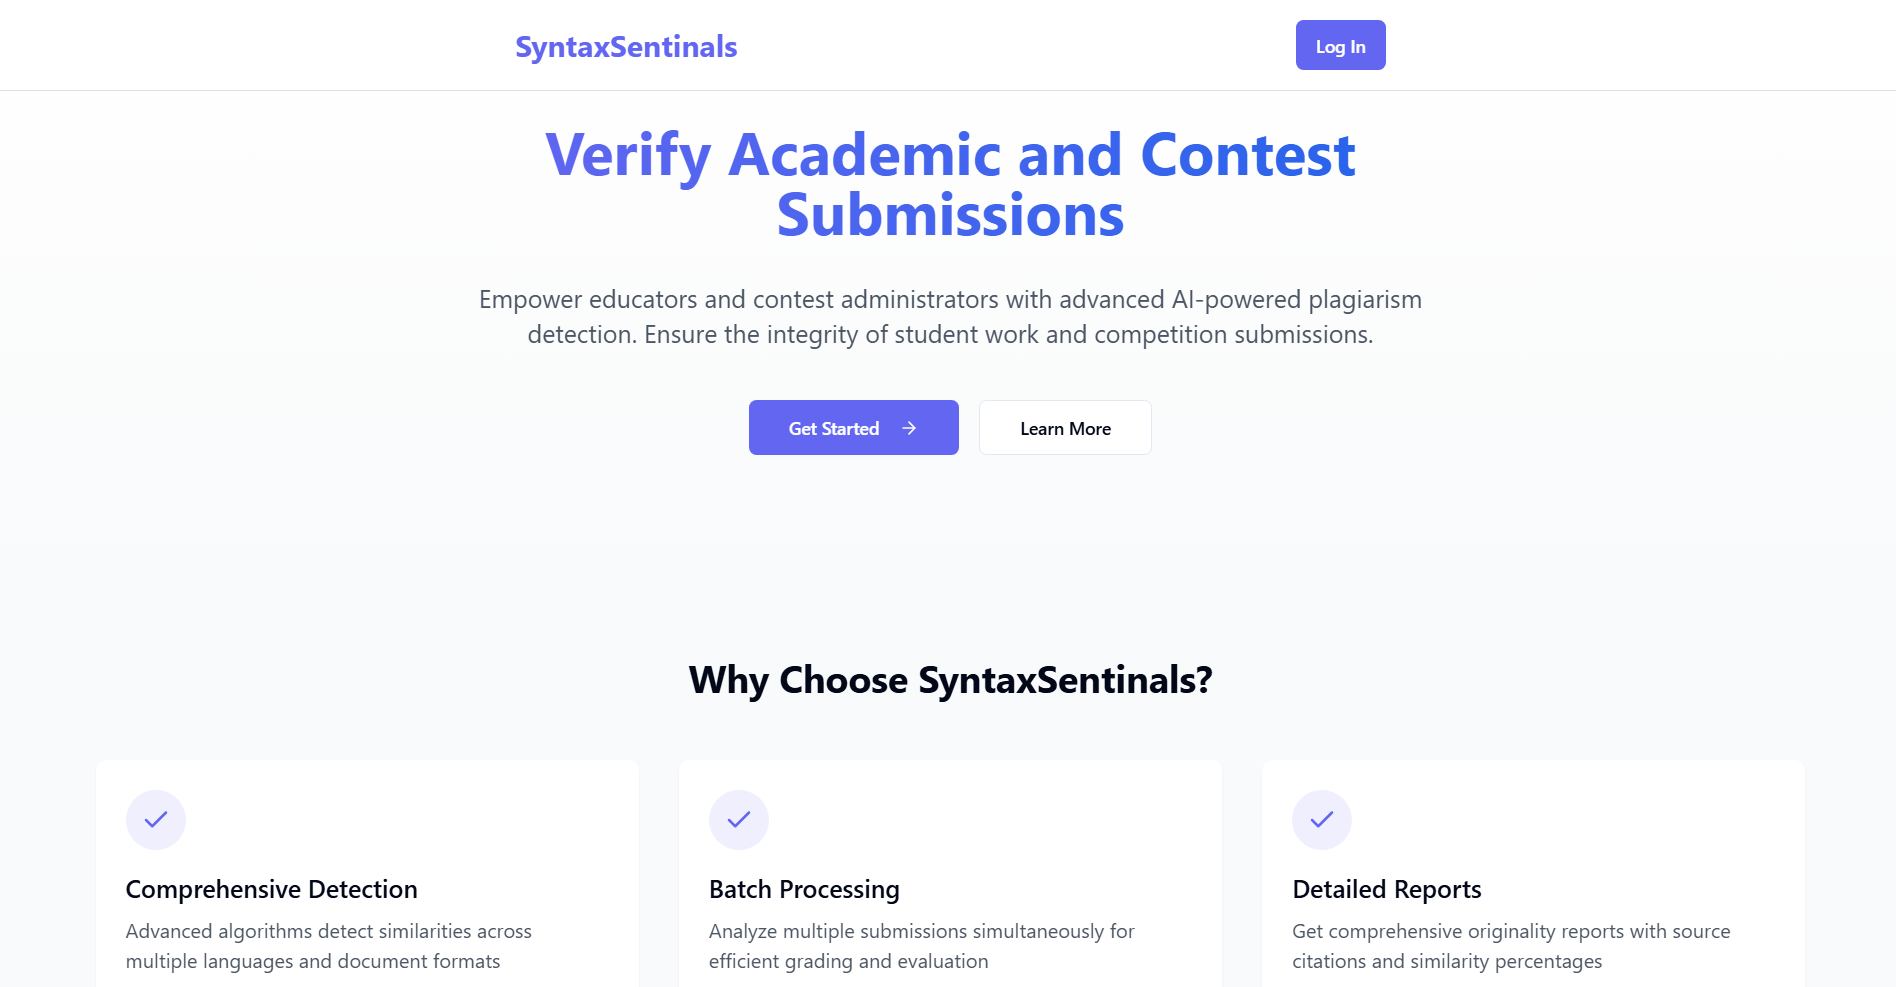
\includegraphics[width=\textwidth]{HomePage.png}
    \caption{Home Page}
    \label{fig:home}
  \end{figure}

Above is our home page, users can login via the Log In button or click on Get Started.

\begin{figure}[H]
    \centering
    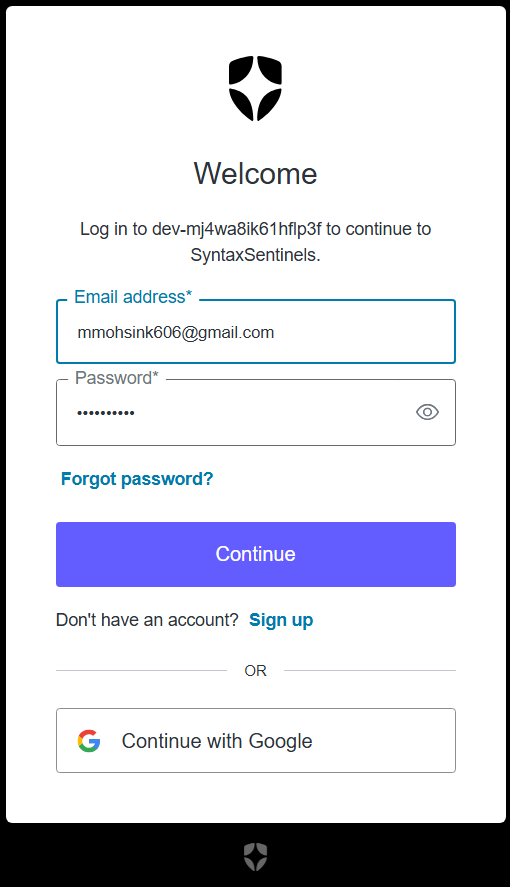
\includegraphics[height=\dimexpr\textheight-5cm\relax]{Login.png}
    \caption{Login Page}
    \label{fig:Login}
  \end{figure}

Above is the login page where users can login via their existing account or sign up via the sign up button.

\begin{figure}[H]
    \centering
    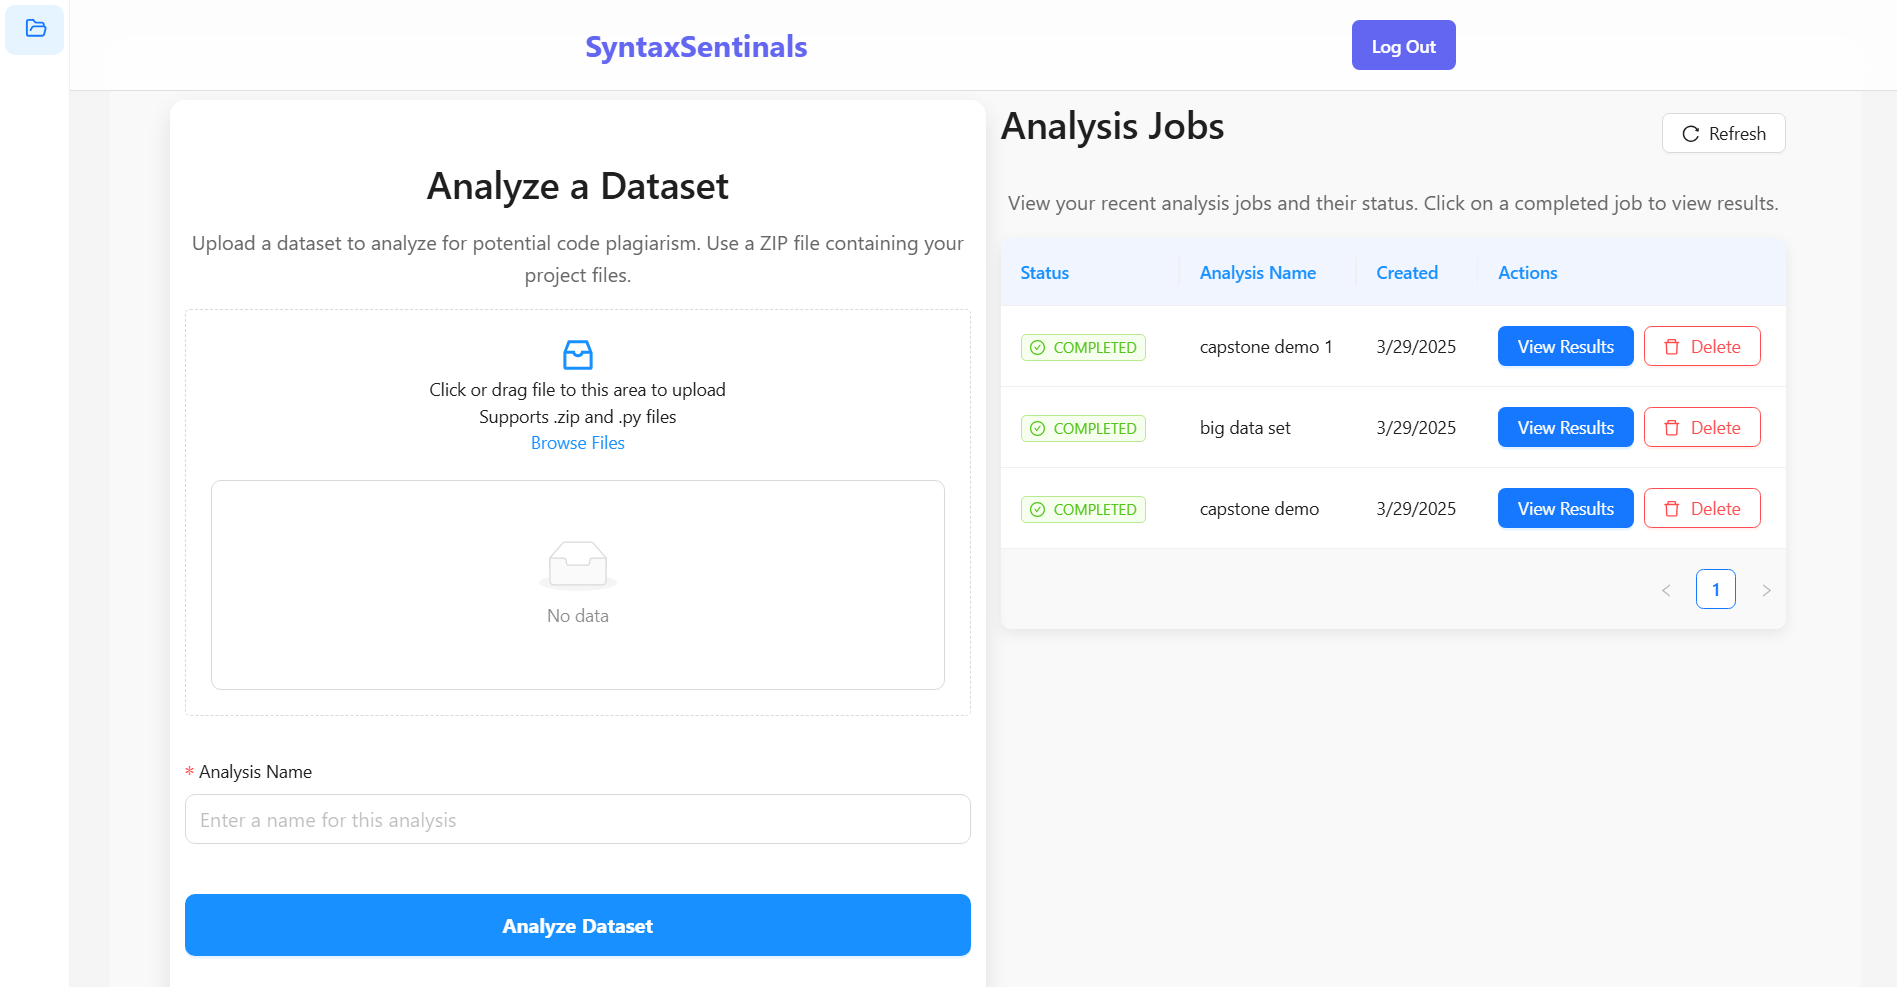
\includegraphics[width=\textwidth]{DashBoard.png}
    \caption{Dashboard Page}
    \label{fig:Dashboard}
  \end{figure}

Above is the dashboard page. On the right users can see a history of their jobs, view the rsults and delete a job and also click on refresh to refresh the analysis list.
On the top, the user can also press Log Out to Log out of the system.
On the left, users can upload files, give the analysis a name and then click on analyze dataset to start the analysis.

\begin{figure}[H]
    \centering
    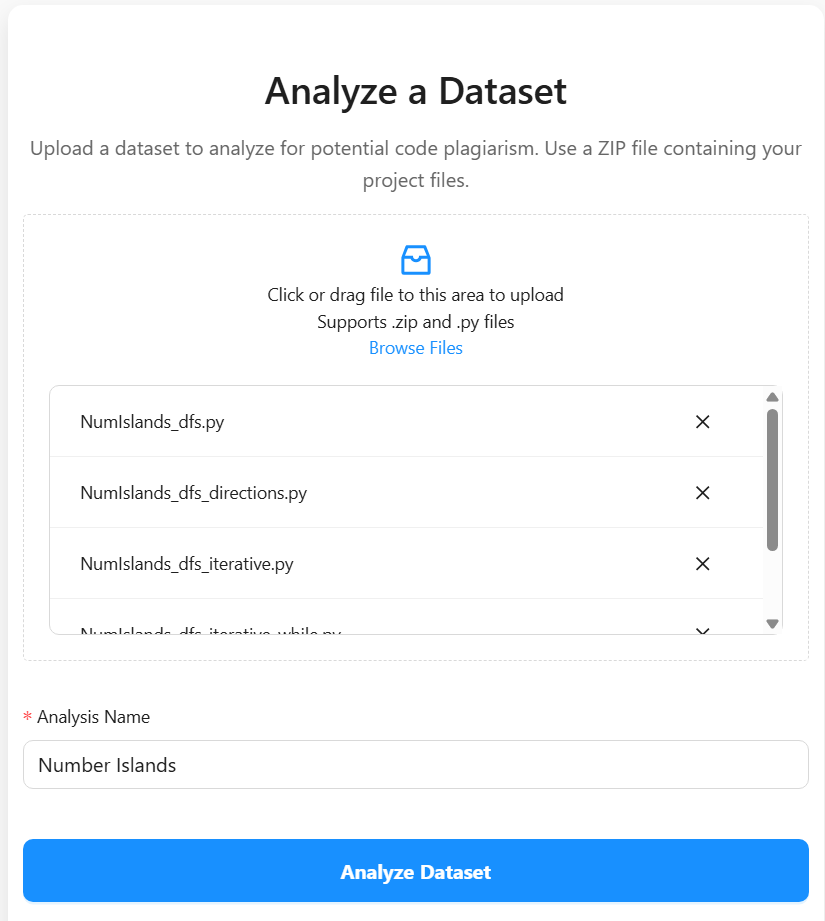
\includegraphics[width=\textwidth]{Analyze.png}
    \caption{example of a dataset}
    \label{fig:Analyze dataset}
  \end{figure}

Above is an example of how files can be uploaded, the name of the analysis can be given and the analyze dataset button can be pressed to start the analysis.

\begin{figure}[H]
    \centering
    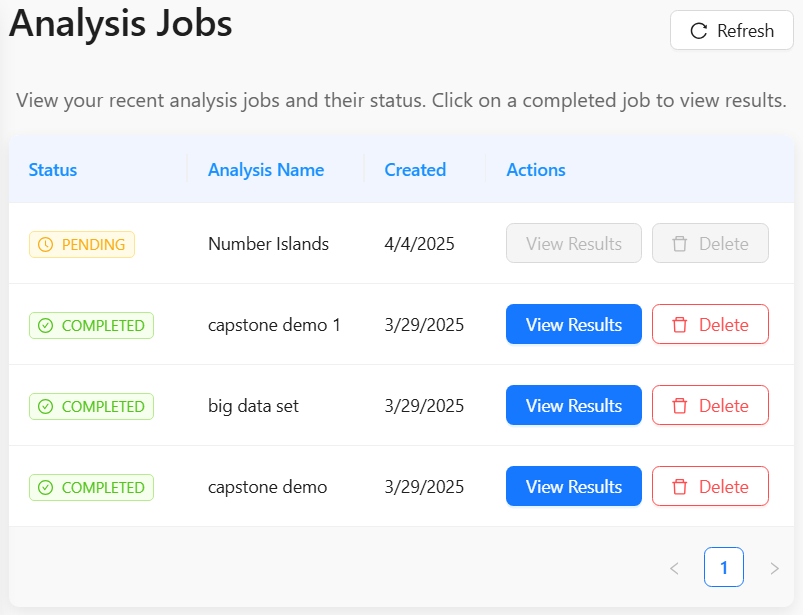
\includegraphics[width=\textwidth]{JobStatus.png}
    \caption{Job Pending Status}
    \label{fig:Job Pending}
  \end{figure}

Once the analysis is submitted, it will be in the pending state as it is waiting for the compute server to pick it up.

\begin{figure}[H]
    \centering
    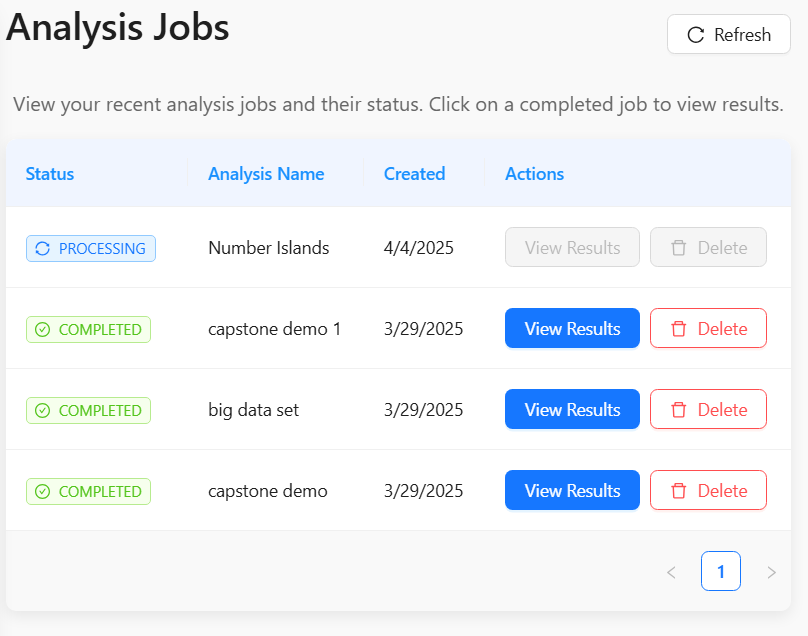
\includegraphics[width=\textwidth]{JobStatusProcessing.png}
    \caption{Job Pending Status}
    \label{fig:Job Processing}
  \end{figure}

Once the compute server picks up the job, it will be in the processing state.

\begin{figure}[H]
    \centering
    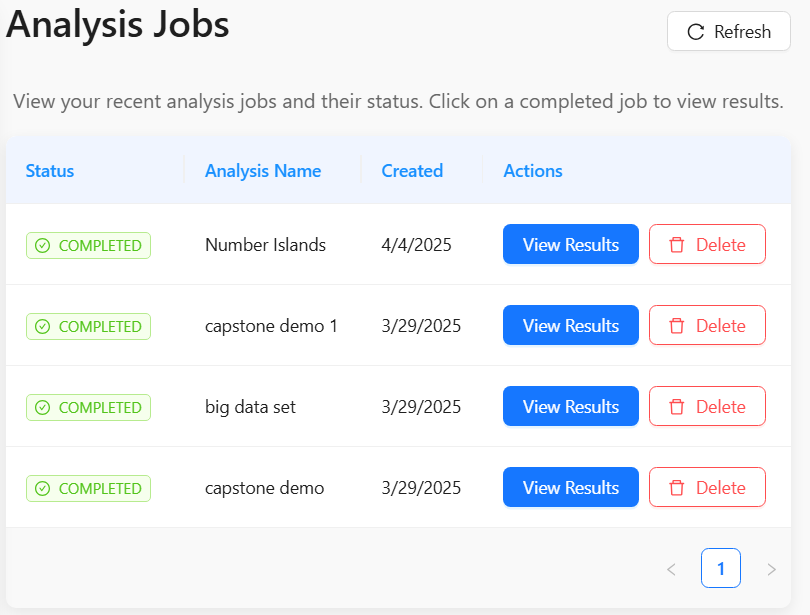
\includegraphics[width=\textwidth]{JobStatusComplete.png}
    \caption{Job Complete Status}
    \label{fig:Job Complete}
  \end{figure}

Once the compute server finishes the job, it will be in the complete state. Users can click on the view results button to see the results of the analysis.

\begin{figure}[H]
    \centering
    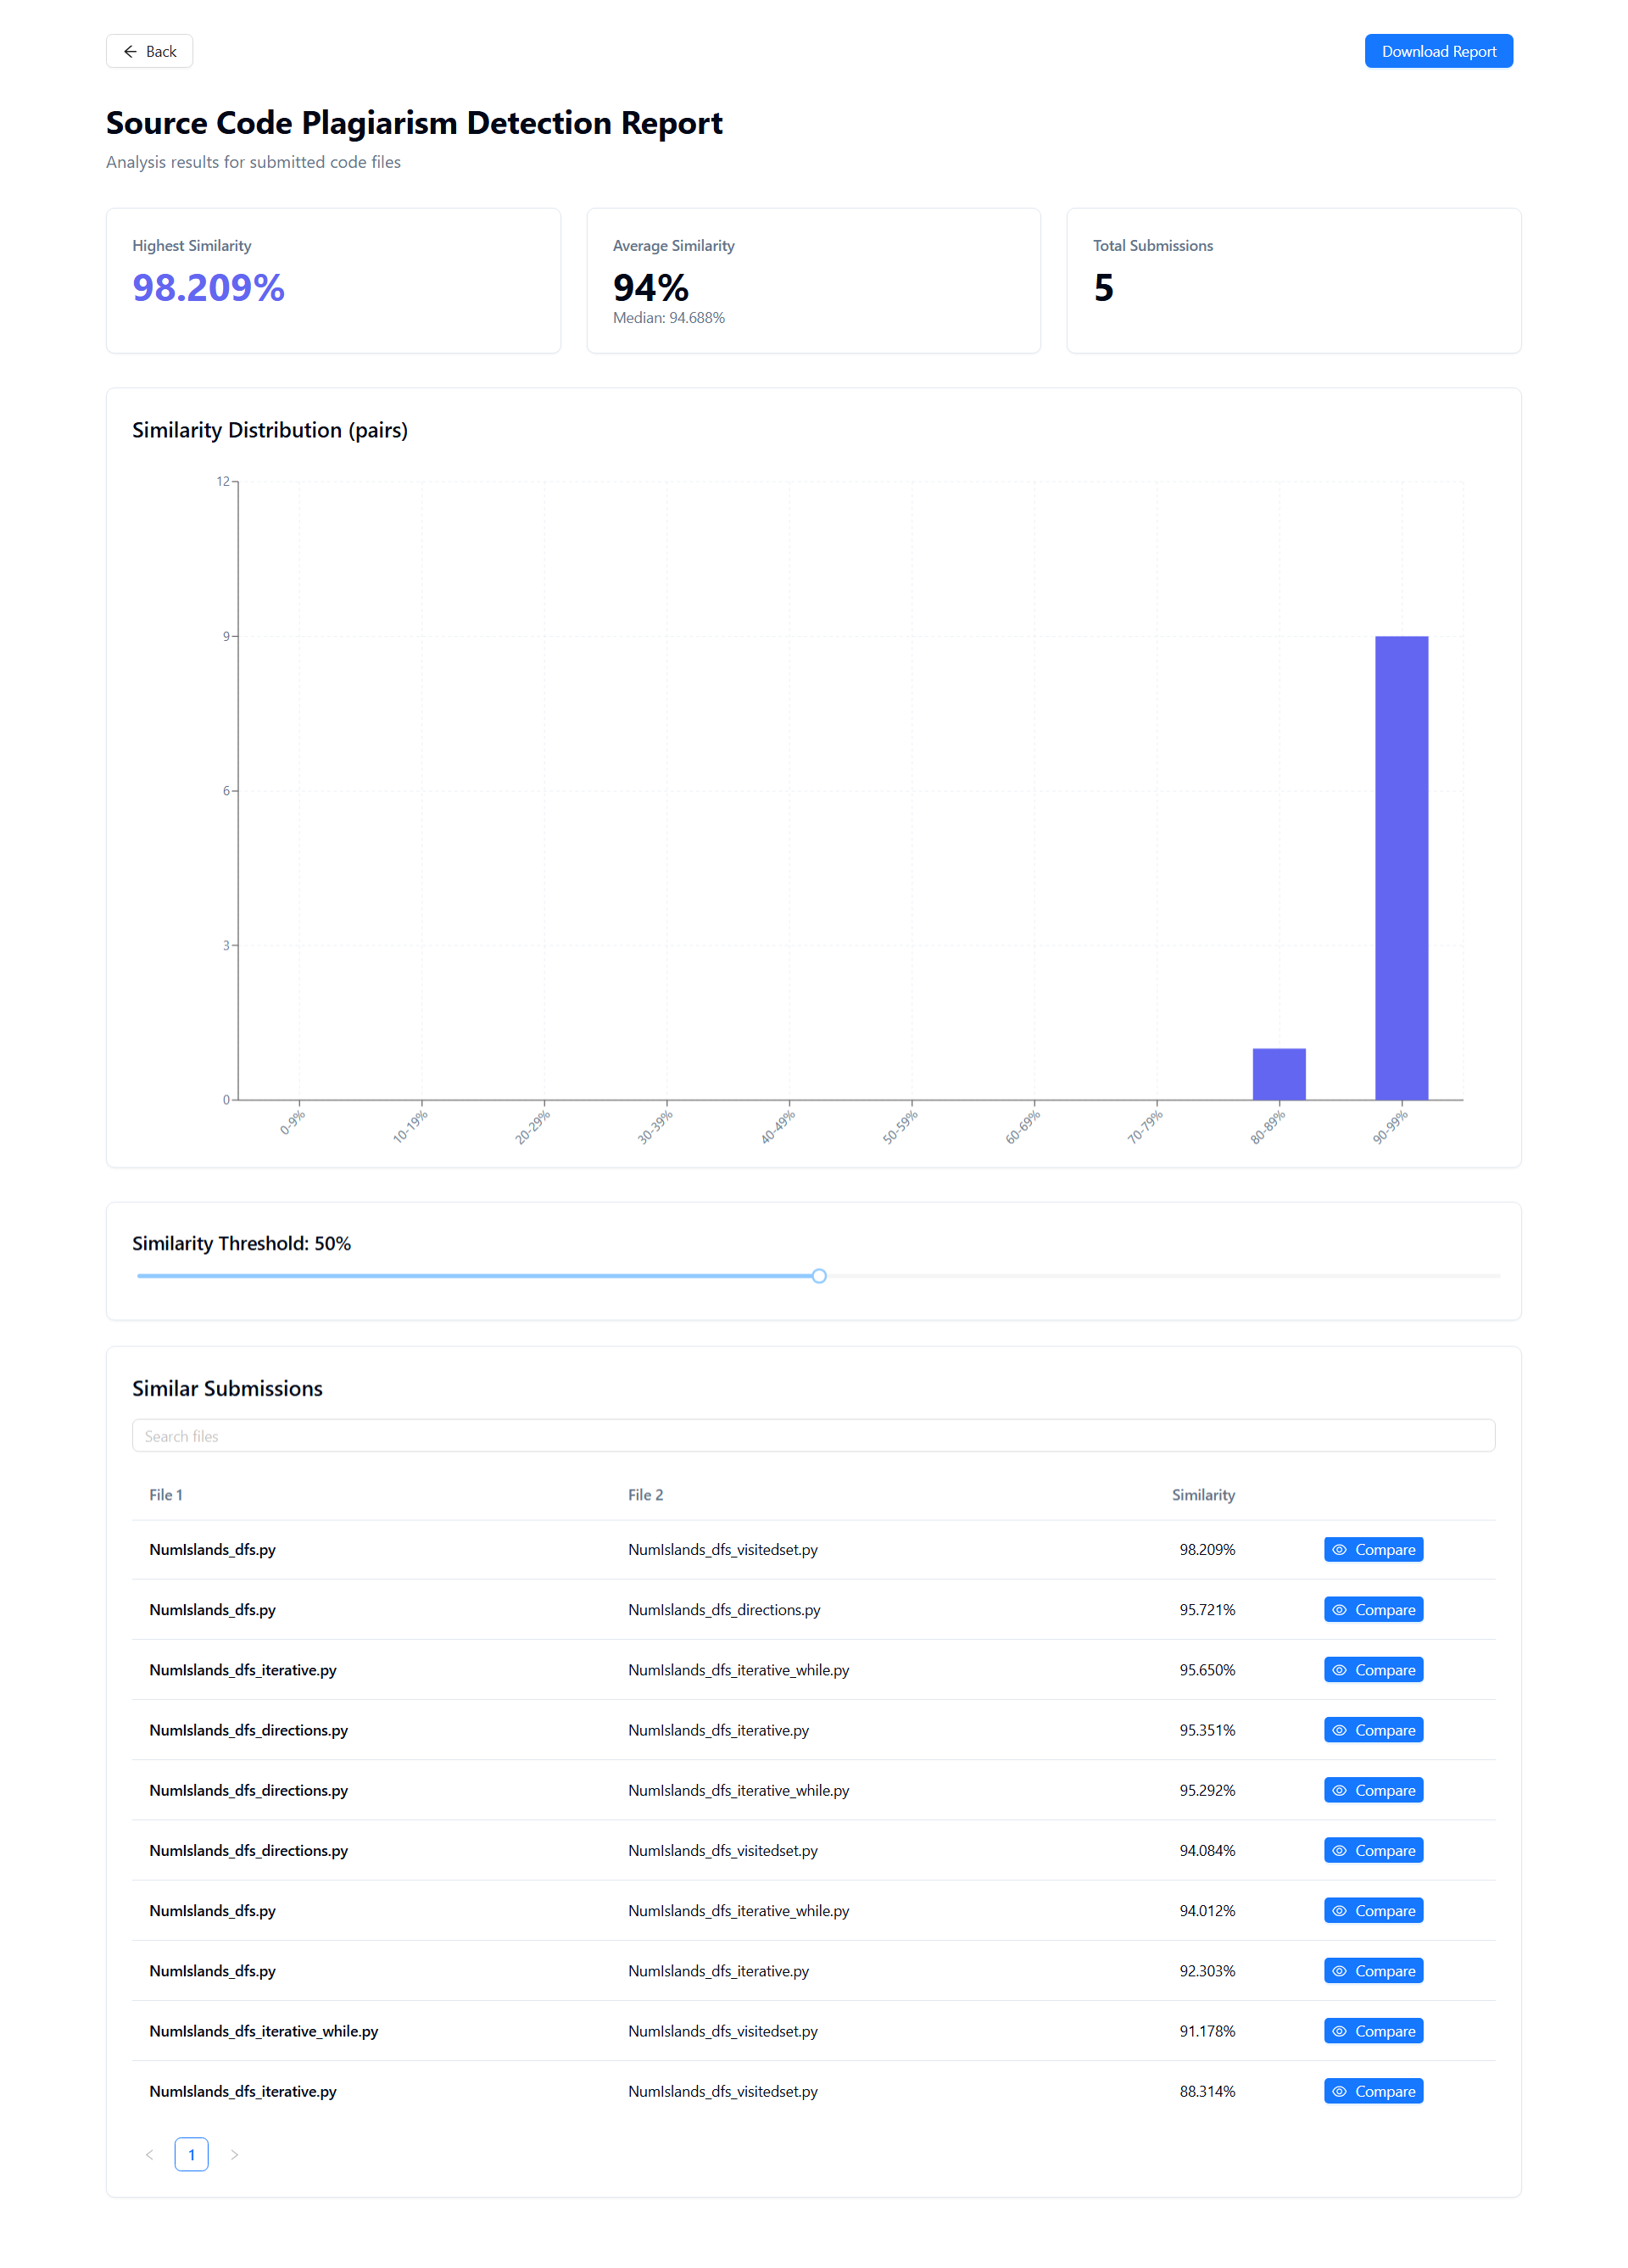
\includegraphics[height=\dimexpr\textheight-1cm\relax]{Results.png}
    \caption{Results Page}
    \label{fig:Results}
  \end{figure}

Above is our results page where users can see the results of their analysis. They can also download the results via the download Report Button.
The scroll bar can be used to filter the file pairs by similarity score and the search bar can filter the files by name.

\begin{figure}[H]
    \centering
    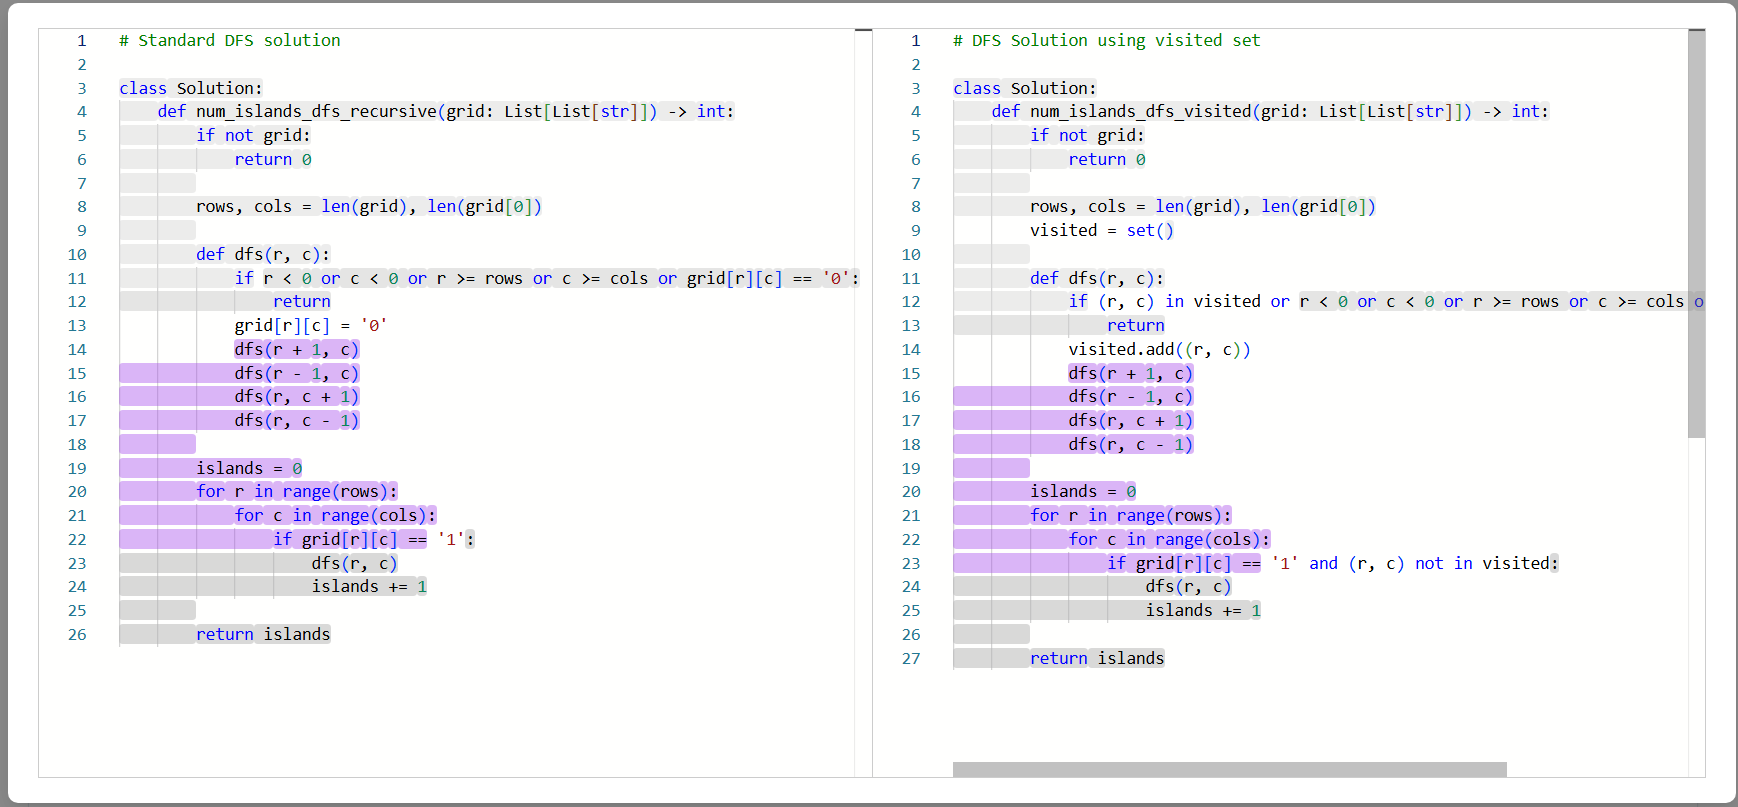
\includegraphics[width=\textwidth]{LineByLine.png}
    \caption{Line by Line Analysis}
    \label{fig:Line by Line}
  \end{figure}

Clicking on compare beside the file pair will take the user to the line by line analysis page where they can see the differences between the two files.
The clusters are differentiated by colour. As can be seen in the example above, the purple cluster on the right hand side is similar to the purple cluster on the left hand side.

\section{Debugging and Troubleshooting}

\subsection*{1. Virtual Environment Issues}
\begin{itemize}
    \item Make sure it's activated. If not:
\begin{Verbatim}[fontsize=\small]
source .venv/bin/activate
\end{Verbatim}
    \item Reinstall dependencies:
\begin{Verbatim}[fontsize=\small]
pip install --force-reinstall -r requirements.txt
\end{Verbatim}
\end{itemize}

\subsection*{2. Node.js Dependency Errors}
\begin{Verbatim}[fontsize=\small]
npm install
rm -rf node_modules
npm cache clean --force
npm install
\end{Verbatim}

\subsection*{3. Environment Variable Issues}
Double-check your \texttt{.env} files. Ensure sensitive values are correctly quoted and loaded.

\subsection*{4. Port Conflicts}
Check which processes are using ports \texttt{3000}, \texttt{3001} and kill or reconfigure as necessary.

\subsection*{5. AWS/Firebase Issues}
Use:
\begin{Verbatim}[fontsize=\small]
aws sts get-caller-identity
\end{Verbatim}

\section{Additional Tips}
\begin{itemize}
    \item Keep documentation updated.
    \item Use Git for configuration tracking.
    \item Backup sensitive files securely.
    \item Test components in isolation.
    \item Mirror environments between dev and prod.
\end{itemize}

\end{document}
